\let\negmedspace\undefined
\let\negthickspace\undefined
\documentclass[journal]{IEEEtran}
\usepackage[a5paper, margin=10mm, onecolumn]{geometry}
%\usepackage{lmodern} % Ensure lmodern is loaded for pdflatex
\usepackage{tfrupee} % Include tfrupee package

\setlength{\headheight}{1cm} % Set the height of the header box
\setlength{\headsep}{0mm}     % Set the distance between the header box and the top of the text

\usepackage{gvv-book}
\usepackage{gvv}
\usepackage{cite}
\usepackage{amsmath,amssymb,amsfonts,amsthm}
\usepackage{algorithmic}
\usepackage{graphicx}
\usepackage{textcomp}
\usepackage{xcolor}
\usepackage{txfonts}
\usepackage{listings}
\usepackage{enumitem}
\usepackage{mathtools}
\usepackage{gensymb}
\usepackage{comment}
%\usepackage{multiclo}
\usepackage[breaklinks=true]{hyperref}
\usepackage{tkz-euclide} 
\usepackage{listings}
% \usepackage{gvv} 
\graphicspath{ {./figs/} }

\begin{document}

\title{
ME: MECHANICAL ENGINEERING}
\author{AI25BTECH11011}
\maketitle
\renewcommand{\thefigure}{\theenumi}
\renewcommand{\thetable}{\theenumi}

\textbf{Q.1 - Q.20 carry one mark each.}

\begin{enumerate}

\item The minimum value of function $ y = x^2 $ in the interval $[1,5]$ is
\begin{multicols}{4}
\begin{enumerate}
\item 0
\item 1
\item 25
\item undefined
\end{enumerate}
\end{multicols}
\hfill (GATE ME 2007)

\item If a square matrix $ A $ is real and symmetric, then the eigenvalues
\begin{multicols}{2}
\begin{enumerate}
\item are always real
\item are always real and positive
\item are always real and non-negative
\item occur in complex conjugate pairs
\end{enumerate}
\end{multicols}
\hfill (GATE ME 2007)

\item If $ (x, y) $ and $ u(x, y) $ are functions with continuous second derivatives, then $ u(x, y) + iv(x, y) $ can be expressed as an analytic function of $ x + iy $ when
\begin{enumerate}
\item $ \frac{\partial u}{\partial x} = \frac{\partial v}{\partial y}, \quad \frac{\partial u}{\partial y} = -\frac{\partial v}{\partial x} $
\item $ \frac{\partial u}{\partial x} = \frac{\partial v}{\partial x}, \quad \frac{\partial u}{\partial y} = \frac{\partial v}{\partial y} $
\item $ \frac{\partial^2 u}{\partial x^2} + \frac{\partial^2 u}{\partial y^2} = 0 $
\item $ \frac{\partial^2 v}{\partial x^2} + \frac{\partial^2 v}{\partial y^2} = 1 $
\end{enumerate}
\hfill (GATE ME 2007)

\item The partial differential equation $ \frac{\partial^2 z}{\partial x^2} + \left( \frac{\partial z}{\partial y} \right)^2 = 3 $ has
\begin{multicols}{2}
\begin{enumerate}
\item degree 1, order 2
\item degree 1, order 1
\item degree 2, order 1
\item degree 2, order 2
\end{enumerate}
\end{multicols}
\hfill (GATE ME 2007)

\item Which of the following relationships is valid only for reversible processes undergone by a closed system of simple compressible substance (neglect changes in kinetic and potential energy)?
\begin{multicols}{2}
\begin{enumerate}
\item $ \delta Q = dU + \delta W $
\item $ T dS = dU + p dV $
\item $ T dS = dU + \delta W $
\item $ \delta Q = dU + p dV $
\end{enumerate}
\end{multicols}
\hfill (GATE ME 2007)

\item Water has a critical specific volume of 0.003155 m³/kg. A closed and rigid steel tank of volume 0.025 m³ contains a mixture of water and steam at 0.1 MPa. The mass of the mixture is 10 kg. The tank is now slowly heated. The liquid level inside the tank
\begin{enumerate}
\item will rise
\item will fall
\item will remain constant
\item may rise or fall depending on the amount of heat transferred
\end{enumerate}
\hfill (GATE ME 2007)

\item Consider an incompressible laminar boundary layer flow over a flat plate of length $ L $, aligned with the direction of an oncoming uniform free stream. If $ F $ is the ratio of the drag force on the front half of the plate to the drag force on the rear half, then
\begin{multicols}{4}
\begin{enumerate}
\item $ F < \frac{1}{2} $
\item $ F = \frac{1}{2} $
\item $ F = 1 $
\item $ F > 1 $
\end{enumerate}
\end{multicols}
\hfill (GATE ME 2007)

\item In a steady flow through a nozzle, the flow velocity on the nozzle axis is given by $ v = U_0(1 + \frac{3x}{L}) \hat{i} $, where $ x $ is the distance along the axis of the nozzle from its inlet plane and $ L $ is the length of the nozzle. The time required for a fluid particle on the axis to travel from the inlet to the exit plane of the nozzle is
\begin{multicols}{4}
\begin{enumerate}
\item $ \frac{L}{U_0} $
\item $ \frac{L}{3U_0} \ln 4 $
\item $ \frac{4L}{3U_0} $
\item $ \frac{L}{2.5U_0} $
\end{enumerate}
\end{multicols}
\hfill (GATE ME 2007)

\item Consider steady laminar incompressible axi-symmetric fully developed viscous flow through a straight circular pipe of constant cross-sectional area at a Reynolds number of 5. The ratio of inertia force to viscous force on a fluid particle is
\begin{multicols}{4}
\begin{enumerate}
\item 5
\item $ \frac{1}{5} $
\item 0
\item $ \infty $
\end{enumerate}
\end{multicols}
\hfill (GATE ME 2007)

\item In a simply-supported beam loaded as shown below, the maximum bending moment in Nm is

\begin{figure}[H]
    \centering
    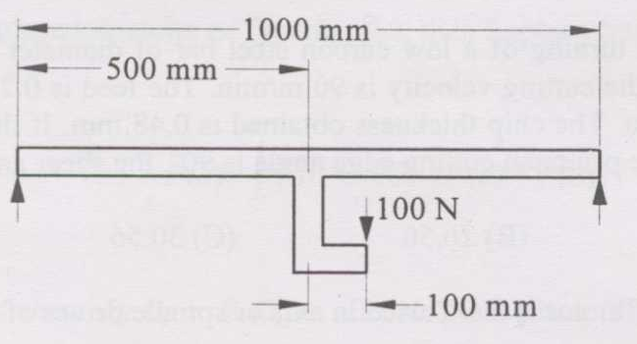
\includegraphics[width=0.8\textwidth]{Fig 1.png}
    \caption{}
    \label{fig:question10}
\end{figure}

\begin{multicols}{4}
\begin{enumerate}
\item 25
\item 30
\item 35
\item 60
\end{enumerate}
\end{multicols}
\hfill (GATE ME 2007)

\item A ball bearing operating at a load $ F $ has 8000 hours of life. The life of the bearing, in hours, when the load is doubled to $ 2F $ is
\begin{multicols}{4}
\begin{enumerate}
\item 8000
\item 6000
\item 4000
\item 1000
\end{enumerate}
\end{multicols}
\hfill (GATE ME 2007)

\item During inelastic collision of two particles, which one of the following is conserved?
\begin{enumerate}
\item total linear momentum only
\item total kinetic energy only
\item both linear momentum and kinetic energy
\item neither linear momentum nor kinetic energy
\end{enumerate}
\hfill (GATE ME 2007)

\item A steel rod of length $ L $ and diameter $ D $, fixed at both ends, is uniformly heated to a temperature rise of $ \Delta T $. The Young's modulus is $ E $ and the coefficient of linear expansion is $ \alpha $. The thermal stress in the rod is
\begin{multicols}{4}
\begin{enumerate}
\item 0
\item $ \alpha \Delta T $
\item $ E \alpha \Delta T $
\item $ \frac{E \alpha \Delta T}{L} $
\end{enumerate}
\end{multicols}
\hfill (GATE ME 2007)

\item For an underdamped harmonic oscillator, resonance
\begin{enumerate}
\item occurs when excitation frequency is greater than undamped natural frequency
\item occurs when excitation frequency is less than undamped natural frequency
\item occurs when excitation frequency is equal to undamped natural frequency
\item never occurs
\end{enumerate}
\hfill (GATE ME 2007)

\item If a particular Fe-C alloy contains less than 0.83% carbon, it is called
\begin{multicols}{2}
\begin{enumerate}
\item high speed steel
\item hypoeutectoid steel
\item hypereutectoid steel
\item cast iron
\end{enumerate}
\end{multicols}
\hfill (GATE ME 2007)

\item Which of the following engineering materials is the most suitable candidate for hot chamber die casting?
\begin{multicols}{2}
\begin{enumerate}
\item low carbon steel
\item titanium
\item copper
\item tin
\end{enumerate}
\end{multicols}
\hfill (GATE ME 2007)

\item Which one of the following is a solid state joining process?
\begin{multicols}{2}
\begin{enumerate}
\item gas tungsten arc welding
\item resistance spot welding
\item friction welding
\item submerged arc welding
\end{enumerate}
\end{multicols}
\hfill (GATE ME 2007)

\item In orthogonal turning of a low carbon steel bar of diameter 150 mm with uncoated carbide tool, the cutting velocity is 90 m/min. The feed is 0.24 mm/rev and the depth of cut is 2 mm. The chip thickness obtained is 0.48 mm. If the orthogonal rake angle is zero and the principal cutting edge angle is 90°, the shear angle in degrees is
\begin{multicols}{4}
\begin{enumerate}
\item 20.56
\item 26.56
\item 30.56
\item 36.56
\end{enumerate}
\end{multicols}
\hfill (GATE ME 2007)

\item Which type of motor is \textbf{NOT}used in axis or spindle drives of CNC machine tools?
\begin{multicols}{2}
\begin{enumerate}
\item induction motor
\item dc servo motor
\item stepper motor
\item linear servo motor
\end{enumerate}
\end{multicols}
\hfill (GATE ME 2007)

\item Volume of a cube of side $ l $ and volume of a sphere of radius $ r $ are equal. Both the cube and the sphere are solid and of same material. They are being cast. The ratio of the solidification time of the cube to that of the sphere is
\begin{multicols}{4}
\begin{enumerate}
\item $ \left( \frac{4\pi}{6} \right)^3 \left( \frac{r}{l} \right)^6 $
\item $ \left( \frac{4\pi}{6} \right) \left( \frac{r}{l} \right)^2 $
\item $ \left( \frac{4\pi}{6} \right) \left( \frac{r}{l} \right)^3 $
\item $ \left( \frac{4\pi}{6} \right)^2 \left( \frac{r}{l} \right)^4 $
\end{enumerate}
\end{multicols}
\hfill (GATE ME 2007)

\begin{center}
\textbf{Q.21 to Q.75 carry two marks each.}
\end{center}

\item If $ y = x + \sqrt{x + \sqrt{x + \sqrt{x + \cdots}}} $, then $ y(2) = $
\begin{multicols}{4}
\begin{enumerate}
\item 4 or 1
\item 4 only
\item 1 only
\item undefined
\end{enumerate}
\end{multicols}
\hfill (GATE ME 2007)

\item The area of a triangle formed by the tips of vectors $ \vec{a}, \vec{b}, \vec{c} $ is
\begin{multicols}{2}
\begin{enumerate}
\item $\dfrac{1}{2} (\vec{a} - \vec{b}) \cdot (\vec{a} - \vec{c})$
\item $\dfrac{1}{2} \left| (\vec{a} - \vec{b}) \times (\vec{a} - \vec{c}) \right|$
\item $\dfrac{1}{2} \left| \vec{a} \times \vec{b} \times \vec{c} \right|$
\item $\dfrac{1}{2} (\vec{a} \times \vec{b}) \cdot \vec{c}$
\end{enumerate}
\end{multicols}
\hfill (GATE ME 2007)

\item The solution of $ \frac{dy}{dx} = y^2 $ with initial value $ y(0) = 1 $ is bounded in the interval
\begin{multicols}{4}
\begin{enumerate}
\item $ -\infty < x < \infty $
\item $ -\infty < x < 1 $
\item $ x < 1, x > 1 $
\item $ -2 \leq x \leq 2 $
\end{enumerate}
\end{multicols}
\hfill (GATE ME 2007)

\item If $ F(s) $ is the Laplace transform of function $ f(t) $, then Laplace transform of $ \int_0^t f(t) dt $ is
\begin{multicols}{4}
\begin{enumerate}
\item $ -F(s) $
\item $ -F(s) - f(0) $
\item $ \frac{F(s)}{s} $
\item $ \int F(s) ds $
\end{enumerate}
\end{multicols}
\hfill (GATE ME 2007)

\item A calculator has accuracy up to 8 digits after decimal place. The value of $ \int_0^1 \sin x \, dx $ when evaluated using this calculator by trapezoidal method with 8 equal intervals, to 5 significant digits is
\begin{multicols}{4}
\begin{enumerate}
\item 0.00000
\item 1.0000
\item 0.00500
\item 0.00025
\end{enumerate}
\end{multicols}
\hfill (GATE ME 2007)

\item Let $ X $ and $ Y $ be two independent random variables. Which one of the relations between expectation (E), variance (Var) and covariance (Cov) given below is FALSE?
\begin{multicols}{2}
\begin{enumerate}
\item $ E(XY) = E(X)E(Y) $
\item $ \text{Cov}(X,Y) = 0 $
\item $ \text{Var}(X+Y) = \text{Var}(X) + \text{Var}(Y) $
\item $ E(X^2Y^2) = (E(X))^2(E(Y))^2 $
\end{enumerate}
\end{multicols}
\hfill (GATE ME 2007)

\item $\lim_{x \to 0} \frac{e^x - \left(1 + x + \frac{x^2}{2}\right)}{x^3} =$
\begin{multicols}{4}
\begin{enumerate}
\item 0
\item $ \frac{1}{6} $
\item $ \frac{1}{3} $
\item 1
\end{enumerate}
\end{multicols}
\hfill (GATE ME 2007)

\item The number of linearly independent eigenvectors of matrix$\myvec{
2 & 0 \\
0 & 2}
$
is
\begin{multicols}{4}
\begin{enumerate}
\item 0
\item 1
\item 2
\item infinite
\end{enumerate}
\end{multicols}
\hfill (GATE ME 2007)

\item The inlet angle of runner blades of a Francis turbine is $ 90^\circ $. The blades are so shaped that the tangential component of velocity at blade outlet is zero. The flow velocity remains constant throughout the blade passage and is equal to half of the blade velocity at runner inlet. The blade efficiency of the runner is
\begin{multicols}{4}
\begin{enumerate}
\item 25\%
\item 50\%
\item 80\%
\item 89\%
\end{enumerate}
\end{multicols}
\hfill (GATE ME 2007)

\item The temperature distribution within the thermal boundary layer over a heated isothermal flat plate is given by $\frac{T - T_w}{T_\infty - T_w} = \frac{3}{2} \left( \frac{y}{\delta_t} \right) - \frac{1}{2} \left( \frac{y}{\delta_t} \right)^3.$ The local Nusselt number based on the thermal boundary layer thickness $ \delta $, is
\begin{multicols}{4}
\begin{enumerate}
\item 1.33
\item 1.50
\item 2.0
\item 4.64
\end{enumerate}
\end{multicols}
\hfill (GATE ME 2007)

\item In a counterflow heat exchanger, hot fluid enters at $ 60^\circ C $ and cold fluid leaves at $ 30^\circ C $. Mass flow rate of the hot fluid is 1 kg/s and that of the cold fluid is 2 kg/s. Specific heat of the hot fluid is 10 kJ/kgK and that of the cold fluid is 5 kJ/kgK. The Log Mean Temperature Difference (LMTD) for the heat exchanger in $ ^\circ C $ is
\begin{multicols}{4}
\begin{enumerate}
\item 15
\item 30
\item 35
\item 45
\end{enumerate}
\end{multicols}
\hfill (GATE ME 2007)

\item The average heat transfer coefficient on a thin hot vertical plate suspended in still air can be determined from observations of the change in plate temperature with time as it cools. Assume the plate temperature to be uniform at any instant of time and radiation heat exchange with the surroundings negligible. The ambient temperature is $ 25^\circ C $, the plate has a total surface area of $ 0.1 \, m^2 $ and a mass of 4 kg. The specific heat of the plate material is 2.5 kJ/kgK. The convective heat transfer coefficient in W/m$^2$K, at the instant when the plate temperature is $ 225^\circ C $ and the change in plate temperature with time $ \frac{dT}{dt} = -0.02 \, K/s $, is
\begin{multicols}{4}
\begin{enumerate}
\item 200
\item 20
\item 15
\item 10
\end{enumerate}
\end{multicols}
\hfill (GATE ME 2007)

\item A model of a hydraulic turbine is tested at a head of 1/4th of that under which the full scale turbine works. The diameter of the model is half of that of the full scale turbine. If $ N $ is the RPM of the full scale turbine, then the RPM of the model will be
\begin{multicols}{4}
\begin{enumerate}
\item $ \frac{N}{4} $
\item $ \frac{N}{2} $
\item $ N $
\item $ 2N $
\end{enumerate}
\end{multicols}
\hfill (GATE ME 2007)

\item The stroke and bore of a four stroke spark ignition engine are 250 mm and 200 mm respectively. The clearance volume is $ 0.001 \, m^3 $. If the specific heat ratio $ \gamma = 1.4 $, the air-standard cycle efficiency of the engine is
\begin{multicols}{4}
\begin{enumerate}
\item 46.40\%
\item 56.10\%
\item 58.20\%
\item 62.80\%
\end{enumerate}
\end{multicols}
\hfill (GATE ME 2007)

\item A building has to be maintained at $ 21^\circ C $ (dry bulb) and $ 14.5^\circ C $ (wet bulb). The dew point temperature under these conditions is $ 10.17^\circ C $. The outside temperature is $ -23^\circ C $ (dry bulb) and the internal and external surface heat transfer coefficients are 8 W/m$^2$K and 23 W/m$^2$K respectively. If the building wall has a thermal conductivity of 1.2 W/mK, the minimum thickness (in m) of the wall required to prevent condensation is
\begin{multicols}{4}
\begin{enumerate}
\item 0.471
\item 0.407
\item 0.321
\item 0.125
\end{enumerate}
\end{multicols}
\hfill (GATE ME 2007)

\item Atmospheric air at a flow rate of 3 kg/s (on dry basis) enters a cooling and dehumidifying coil with an enthalpy of 85 kJ/kg of dry air and a humidity ratio of 19 grams/kg of dry air. The air leaves the coil with an enthalpy of 43 kJ/kg of dry air and a humidity ratio of 8 grams/kg of dry air. If the condensate water leaves the coil with an enthalpy of 67 kJ/kg, the required cooling capacity of the coil in kW is
\begin{multicols}{4}
\begin{enumerate}
\item 75.0
\item 123.8
\item 128.2
\item 159.0
\end{enumerate}
\end{multicols}
\hfill (GATE ME 2007)

\item A heat transformer is a device that transfers a part of the heat, supplied to it at an intermediate temperature, to a high temperature reservoir while rejecting the remaining part to a low temperature heat sink. In such a heat transformer, 100 kJ of heat is supplied at 350 K. The maximum amount of heat in kJ that can be transferred to 400 K, when the rest is rejected to a heat sink at 300 K is
\begin{multicols}{4}
\begin{enumerate}
\item 12.50
\item 14.29
\item 33.33
\item 57.14
\end{enumerate}
\end{multicols}
\hfill (GATE ME 2007)

\item Which combination of the following statements is correct?

The incorporation of reheater in a steam power plant:

P: always increases the thermal efficiency of the plant.

Q: always increases the dryness fraction of steam at condenser inlet.

R: always increases the mean temperature of heat addition. 

S: always increases the specific work output.

\begin{multicols}{4}
\begin{enumerate}
\item P and S
\item Q and S
\item P, R and S
\item P, Q, R and S
\end{enumerate}
\end{multicols}
\hfill (GATE ME 2007)

\item Which combination of the following statements is correct? 

P: A gas cools upon expansion only when its Joule-Thomson coefficient is positive in the temperature range of expansion.

Q: For a system undergoing a process, its entropy remains constant only when the process is reversible.  

R: The work done by a closed system in an adiabatic process is a point function.  

S: A liquid expands upon freezing when the slope of its fusion curve on Pressure-Temperature diagram is negative.

\begin{multicols}{4}
\begin{enumerate}
\item R and S
\item P and Q
\item Q, R and S
\item P, Q and R
\end{enumerate}
\end{multicols}
\hfill (GATE ME 2007)

\item Which combination of the following statements about steady incompressible forced vortex flow is correct?

P: Shear stress is zero at all points in the flow.

Q: Vorticity is zero at all points in the flow.

R: Velocity is directly proportional to the radius from the centre of the vortex.  

S: Total mechanical energy per unit mass is constant in the entire flow field.

\begin{multicols}{4}
\begin{enumerate}
\item P and Q
\item R and S
\item P and R
\item P and S
\end{enumerate}
\end{multicols}
\hfill (GATE ME 2007)

\item Match the items in columns I and II. 

\begin{tabular}{cc}
\textbf{Column 1}         & \textbf{Column 2}\\
P: Centrifugal compressor & 1: Axial flow \\
Q: Centrifugal pump       & 2: Surging \\ 
R: Pelton wheel           & 3: Priming \\  
S: Kaplan turbine         & 4: Pure impulse \\ 
\end{tabular}

\begin{multicols}{2}
\begin{enumerate}
\item P-2, Q-3, R-4, S-1
\item P-2, Q-3, R-1, S-4
\item P-3, Q-4, R-1, S-2
\item P-1, Q-2, R-3, S-4
\end{enumerate}
\end{multicols}
\hfill (GATE ME 2007)

\item A uniformly loaded propped cantilever beam and its free body diagram are shown below. The reactions are  
$ R_1, R_2 $ and moment $ M $

\begin{figure}[H]
    \centering
    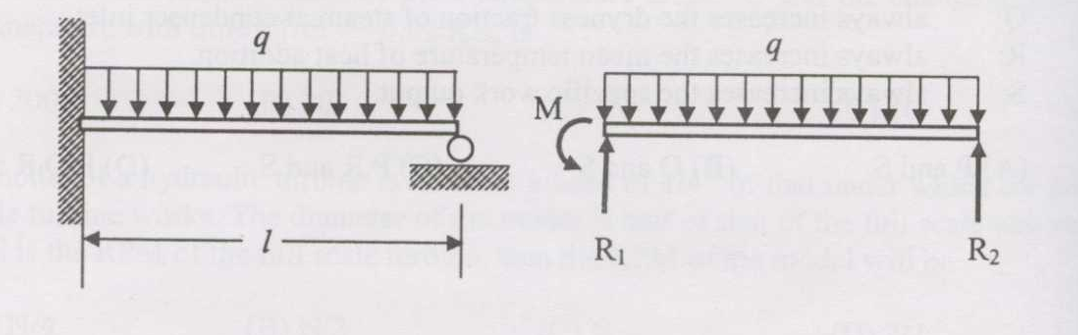
\includegraphics[width=0.8\textwidth]{Fig 2.png}
    \caption{}
    \label{fig:question42}
\end{figure}

\begin{multicols}{2}
\begin{enumerate}
\item $ R_1 = 5qL, R_2 = 3qL, M = 12 $
\item $ R_1 = 3qL, R_2 = 5qL, M = 9qL $
\item $ R_1 = 5qL, R_2 = 3qL, M = 0 $
\item $ R_1 = 3qL, R_2 = 5qL, M = 0 $
\end{enumerate}
\end{multicols}
\hfill (GATE ME 2007)

\item A block of mass $ M $ is released from point $ P $ on a rough inclined plane with inclination angle $ \theta $. The coefficient of friction is $ \mu $. If $ \mu < \tan \theta $, then the time taken by the block to reach another point $ Q $ on the inclined plane, where $ PQ = s $, is

\begin{figure}[H]
    \centering
    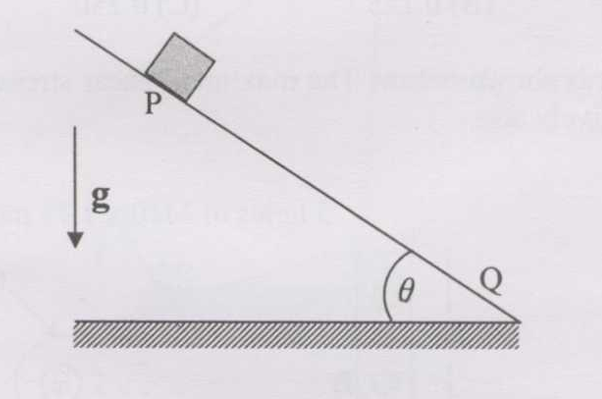
\includegraphics[width=0.8\textwidth]{Fig 3.png}
    \caption{}
    \label{fig:question43}
\end{figure}

\begin{multicols}{2}
\begin{enumerate}
\item $ \sqrt{\frac{2s}{g \cos \theta (\tan \theta - \mu)}} $
\item $ \sqrt{\frac{2s}{g \cos \theta (\tan \theta + \mu)}} $
\item $ \sqrt{\frac{2s}{g \sin \theta (\tan \theta - 1)}} $
\item $ \sqrt{\frac{2s}{g \sin \theta (\tan \theta + 1)}} $
\end{enumerate}
\end{multicols}
\hfill (GATE ME 2007)

\item A 200 × 100 × 50 mm steel block is subjected to a hydrostatic pressure of 15 MPa. The Young’s modulus and Poisson’s ratio of the material are 200 GPa and 0.3 respectively. The change in the volume of the block in mm$^3$ is
\begin{multicols}{4}
\begin{enumerate}
\item 85
\item 90
\item 100
\item 110
\end{enumerate}
\end{multicols}
\hfill (GATE ME 2007)

\item A stepped steel shaft shown below is subjected to 10 Nm torque. If the modulus of rigidity is 80 GPa, the strain energy in the shaft in N·mm is

\begin{figure}[H]
    \centering
    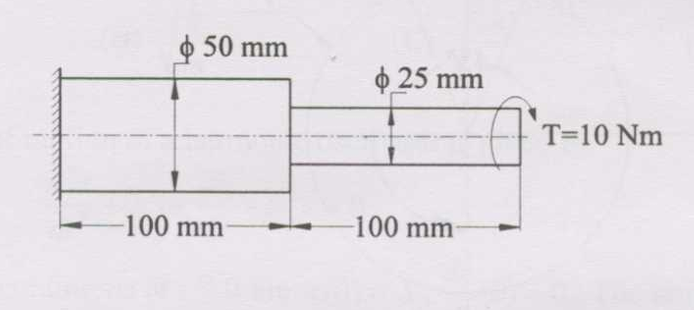
\includegraphics[width=0.8\textwidth]{Fig 4.png}
    \caption{}
    \label{fig:question45}
\end{figure}

\begin{multicols}{4}
\begin{enumerate}
\item 4.12
\item 3.46
\item 1.73
\item 0.86
\end{enumerate}
\end{multicols}
\hfill (GATE ME 2007)

\item A thin spherical pressure vessel of 200 mm diameter and 1 mm thickness is subjected to an internal pressure varying from 4 to 8 MPa. Assume that the yield, ultimate, and endurance strength of material are 600, 800 and 400 MPa respectively. The factor of safety as per Goodman’s relation is
\begin{multicols}{4}
\begin{enumerate}
\item 2.0
\item 1.6
\item 1.4
\item 1.2
\end{enumerate}
\end{multicols}
\hfill (GATE ME 2007)

\item A natural feed journal bearing of diameter 50 mm and length 50 mm operating at 20 revolutions/second carries a load of 2.0 kN. The lubricant used has a viscosity of 20 mPa·s. The radial clearance is 50 µm. The Sommerfeld number for the bearing is
\begin{multicols}{4}
\begin{enumerate}
\item 0.062
\item 0.125
\item 0.250
\item 0.785
\end{enumerate}
\end{multicols}
\hfill (GATE ME 2007)

\item A bolted joint is shown below. The maximum shear stress, in MPa, in the bolts at A and B, respectively are

\begin{figure}[H]
    \centering
    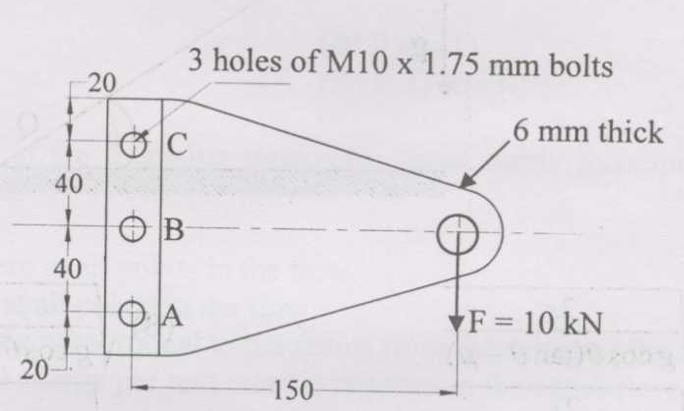
\includegraphics[width=0.8\textwidth]{Fig 5.png}
    \caption{(all dimensions in the figure are in mm)}
    \label{fig:question48}
\end{figure}

\begin{multicols}{2}
\begin{enumerate}
\item 242.6, 42.5
\item 42.5, 242.6
\item 42.5, 42.5
\item 242.6, 242.6
\end{enumerate}
\end{multicols}
\hfill (GATE ME 2007)

\item A block-brake shown below has a face width of 300 mm and a mean coefficient of friction of 0.25. For an activating force of 400 N, the braking torque in Nm is

\begin{figure}[H]
    \centering
    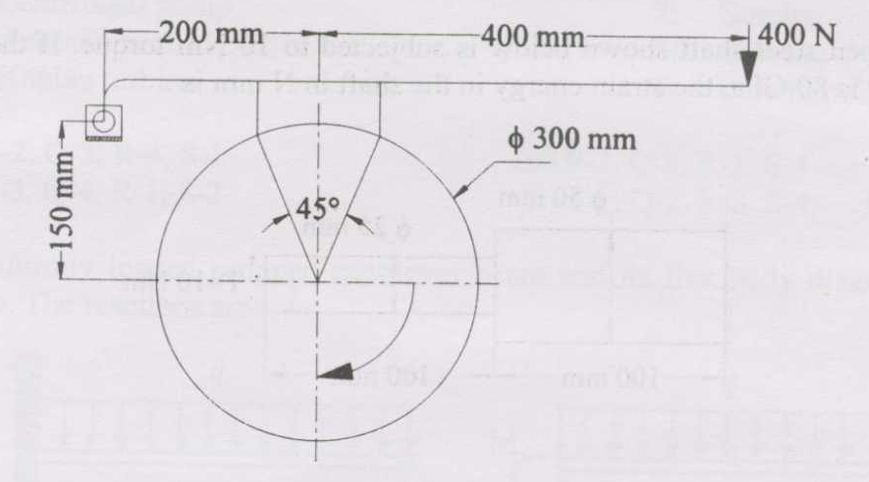
\includegraphics[width=0.8\textwidth]{Fig 6.png}
    \caption{}
    \label{fig:question49}
\end{figure}

\begin{multicols}{4}
\begin{enumerate}
\item 30
\item 40
\item 45
\item 60
\end{enumerate}
\end{multicols}
\hfill (GATE ME 2007)

\item The input link $ O_2P $ of a four bar linkage is rotated at 2 rad/s in counter clockwise direction as shown below. The angular velocity of the coupler $ PQ $ in rad/s, at an instant when $ \angle O_2O_4P = 180^\circ $, is

\begin{figure}[H]
    \centering
    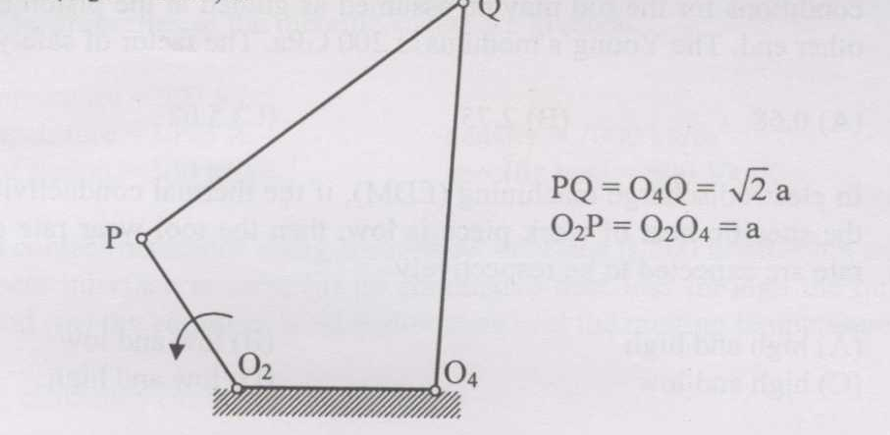
\includegraphics[width=0.8\textwidth]{Fig 7.png}
    \caption{}
    \label{fig:question50}
\end{figure}

\begin{multicols}{4}
\begin{enumerate}
\item 4
\item $ 2\sqrt{2} $
\item 1
\item $ \frac{1}{\sqrt{2}} $
\end{enumerate}
\end{multicols}
\hfill (GATE ME 2007)

\item The speed of an engine varies from 210 rad/s to 190 rad/s. During a cycle the change in kinetic energy is found to be 400 Nm. The inertia of the flywheel in kg·m$^2$ is
\begin{multicols}{4}
\begin{enumerate}
\item 0.10
\item 0.20
\item 0.30
\item 0.40
\end{enumerate}
\end{multicols}
\hfill (GATE ME 2007)

\item The natural frequency of the system shown below is

\begin{figure}[H]
    \centering
    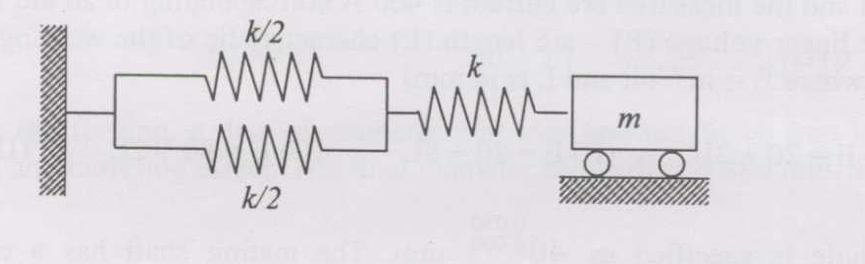
\includegraphics[width=0.8\textwidth]{Fig 8.png}
    \caption{}
    \label{fig:question52}
\end{figure}

\begin{multicols}{4}
\begin{enumerate}
\item $ \sqrt{\frac{k}{2m}} $
\item $ \sqrt{\frac{k}{m}} $
\item $ \sqrt{\frac{2k}{m}} $
\item $ \sqrt{\frac{3k}{m}} $
\end{enumerate}
\end{multicols}
\hfill (GATE ME 2007)

\item The equation of motion of a harmonic oscillator is given by  
\[\frac{dx^2}{dt^2} + 2\zeta \omega_n \frac{dx}{dt} + \omega_n^2 x = 0,\]  
and the initial conditions at $ t = 0 $ are $ x(0) = X, \frac{dx}{dt}(0) = 0 $. The amplitude of $ x(t) $ after $ n $ complete cycles is

\begin{multicols}{2}
\begin{enumerate}
\item $ Xe^{-2\pi \left( \frac{\zeta}{\sqrt{1 - \zeta^2}} \right)} $
\item $ Xe^{2\pi \left( \frac{\zeta}{\sqrt{1 - \zeta^2}} \right)} $
\item $ Xe^{-2\pi \left( \frac{\sqrt{1 - \zeta^2}}{\zeta} \right)} $
\item $ X $
\end{enumerate}
\end{multicols}
\hfill (GATE ME 2007)

\item The piston rod of diameter 20 mm and length 700 mm in a hydraulic cylinder is subjected to a compressive force of 10 kN due to the internal pressure. The end conditions for the rod may be assumed as guided at the piston end and hinged at the other end. The Young’s modulus is 200 GPa. The factor of safety for the piston rod is
\begin{multicols}{4}
\begin{enumerate}
\item 0.68
\item 2.75
\item 5.62
\item 11.0
\end{enumerate}
\end{multicols}
\hfill (GATE ME 2007)

\item In electrodischarge machining (EDM), if the thermal conductivity of tool is high and the specific heat of work piece is low, then the tool wear rate and material removal rate are expected to be respectively
\begin{multicols}{2}
\begin{enumerate}
\item high and high
\item low and low
\item high and low
\item low and high
\end{enumerate}
\end{multicols}
\hfill (GATE ME 2007)

\item In orthogonal turning of medium carbon steel, the specific machining energy is 2.0 J/mm$^3$. The cutting velocity, feed and depth of cut are 120 m/min, 0.2 mm/rev and 2 mm respectively. The main cutting force in N is
\begin{multicols}{4}
\begin{enumerate}
\item 40
\item 80
\item 400
\item 800
\end{enumerate}
\end{multicols}
\hfill (GATE ME 2007)

\item A direct current welding machine with a linear power source characteristic provides open circuit voltage of 80 V and short circuit current of 800 A. During welding with the machine, the measured arc current is 500 A corresponding to an arc length of 5.0 mm and the measured arc current is 460 A corresponding to an arc length of 7.0 mm. The linear voltage (E) – arc length (L) characteristic of the welding arc can be given as (where E is in Volt and L is in mm)
\begin{multicols}{4}
\begin{enumerate}
\item $ E = 20 + 2L $
\item $ E = 20 + 8L $
\item $ E = 80 + 2L $
\item $ E = 80 + 8L $
\end{enumerate}
\end{multicols}
\hfill (GATE ME 2007)

\item A hole is specified as 400.000 mm. The mating shaft has a clearance fit with minimum clearance of 0.01 mm. The tolerance on the shaft is 0.04 mm. The maximum clearance in mm between the hole and the shaft is
\begin{multicols}{4}
\begin{enumerate}
\item 0.04
\item 0.05
\item 0.10
\item 0.11
\end{enumerate}
\end{multicols}
\hfill (GATE ME 2007)

\item In orthogonal turning of low carbon steel pipe with principal cutting edge angle of $ 90^\circ $, the main cutting force is 1000 N and the feed force is 800 N. The shear angle is $ 25^\circ $ and orthogonal rake angle is zero. Employing Merchant’s theory, the ratio of friction force to normal force acting on the cutting tool is
\begin{multicols}{4}
\begin{enumerate}
\item 1.56
\item 1.25
\item 0.80
\item 0.64
\end{enumerate}
\end{multicols}
\hfill (GATE ME 2007)

\item Two metallic sheets, each of 2.0 mm thickness, are welded in a lap joint configuration by resistance spot welding at a welding current of 10 kA and welding time of 10 milliseconds. A spherical fusion zone extending up to the full thickness of each sheet is formed. The properties of the metallic sheets are given as:

ambient temperature = 293 K

melting temperature = 1793 K

latent heat of fusion = 300 kJ/kg

density = 7000 kg/m$^3$

specific heat = 800 J/kg·K

Assume:
(i)contact resistance along sheet-sheet interface is 500 $ \mu\Omega $ and along electrode-sheet interface is zero;
(ii)no conductive heat loss through the bulk sheet materials;
(iii)the complete weld fusion zone is at the melting temperature.

The melting efficiency (in \%) of the process is
\begin{multicols}{4}
\begin{enumerate}
\item 50.37
\item 60.37
\item 70.37
\item 80.37
\end{enumerate}
\end{multicols}
\hfill (GATE ME 2007)

\item Capacities of production of an item over 3 consecutive months in regular time are 100, 100 and 80 and in overtime are 20, 20 and 40. The demands over those 3 months are 90, 130 and 110. The cost of production in regular time and overtime are respectively Rs. 20 per item and Rs. 24 per item. Inventory carrying cost is Rs. 2 per item per month. The levels of starting and final inventory are nil. Backorder is not permitted. For minimum cost of plan, the level of planned production in overtime in the third month is
\begin{multicols}{4}
\begin{enumerate}
\item 40
\item 30
\item 20
\item 0
\end{enumerate}
\end{multicols}
\hfill (GATE ME 2007)

\item In open-die forging, a disc of diameter 200 mm and height 60 mm is compressed without any barreling effect. The final diameter of the disc is 400 mm. The true strain is
\begin{multicols}{4}
\begin{enumerate}
\item 1.986
\item 1.686
\item 1.386
\item 0.602
\end{enumerate}
\end{multicols}
\hfill (GATE ME 2007)

\item The thickness of a metallic sheet is reduced from an initial value of 16 mm to a final value of 10 mm in one single pass rolling with a pair of cylindrical rollers each of diameter of 400 mm. The bite angle in degree will be
\begin{multicols}{4}
\begin{enumerate}
\item 5.936
\item 7.936
\item 8.936
\item 9.936
\end{enumerate}
\end{multicols}
\hfill (GATE ME 2007)

\item Match the correct combination for following metal working processes.  

\begin{tabular}{cc}
\textbf{Processes} & \textbf{Associated state of stress} \\
P. Blanking        & 1.Tension \\
Q. Stretch Forming & 2. Compression \\ 
R. Coining         & 3. Shear \\  
S. Deep Drawing    & 4. Tension and Compression \\
                   & 5. Tension and Shear \\
\end{tabular}

\begin{multicols}{2}
\begin{enumerate}
\item P-2, Q-1, R-3, S-4
\item P-3, Q-4, R-1, S-5
\item P-5, Q-4, R-3, S-1
\item P-3, Q-1, R-2, S-4
\end{enumerate}
\end{multicols}
\hfill (GATE ME 2007)

\item A 200 mm long down sprue has an area of cross-section of 650 mm$^2$ where the pouring basin meets the down sprue (i.e. at the beginning of the down sprue). A constant head of molten metal is maintained by the pouring basin. The molten metal flow rate is $ 6.5 \times 10^5 $ mm$^3$/s. Considering the end of down sprue to be open to atmosphere and an acceleration due to gravity of $ 10^4 $ mm/s$^2$, the area of the down sprue in mm$^2$ at its end (avoiding aspiration effect) should be

\begin{figure}[H]
    \centering
    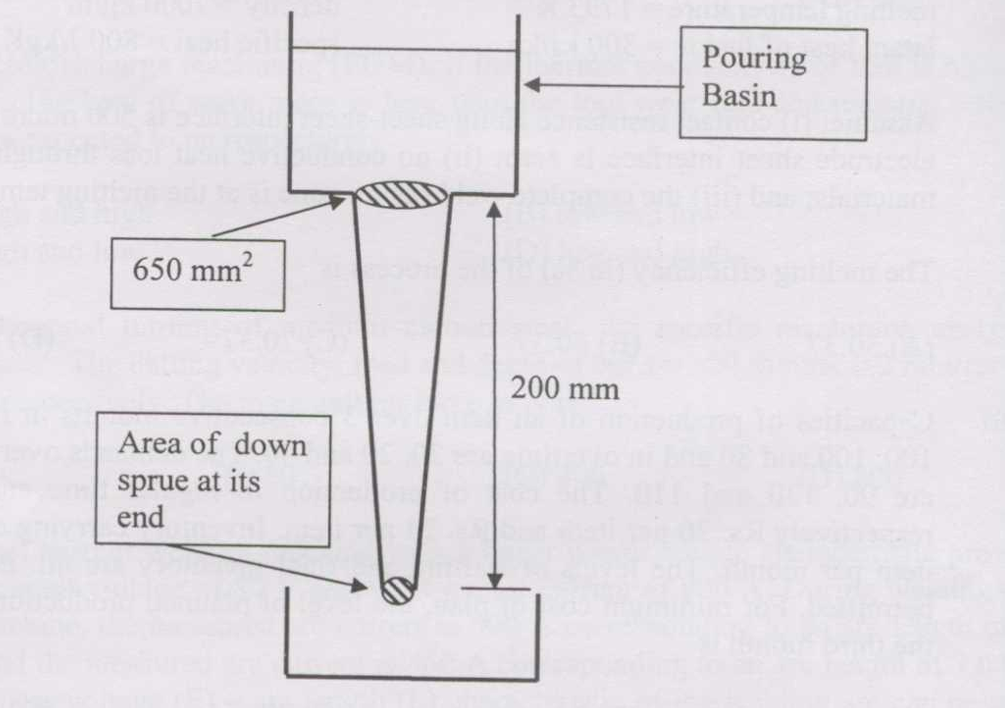
\includegraphics[width=0.8\textwidth]{Fig 9.png}
    \caption{}
    \label{fig:question65}
\end{figure}

\begin{multicols}{4}
\begin{enumerate}
\item 650.0
\item 350.0
\item 290.7
\item 190.0
\end{enumerate}
\end{multicols}
\hfill (GATE ME 2007)

\item The force requirement in a blanking operation of low carbon steel sheet is 5.0 kN. The thickness of the sheet is $ t $ and diameter of the blanked part is $ d $. For the same work material, if the diameter of the blanked part is increased to $ 1.5d $ and thickness is reduced to $ 0.4t $, the new blanking force in kN is
\begin{multicols}{4}
\begin{enumerate}
\item 3.0
\item 4.5
\item 5.0
\item 8.0
\end{enumerate}
\end{multicols}
\hfill (GATE ME 2007)

\item Match the most suitable manufacturing processes for the following parts.

\begin{tabular}{cc}
\textbf{Parts}                  & \textbf{Manufacturing Processes} \\ 
P. Computer chip                & 1. Electrochemical Machining \\
Q. Metal forming dies and molds & 2. Ultrasonic Machining \\
R. Turbine blade                & 3. Electrodischarge Machining \\
S. Glass                        & 4. Photochemical Machining \\
\end{tabular}

\begin{multicols}{2}
\begin{enumerate}
\item P-4, Q-3, R-1, S-2
\item P-4, Q-3, R-2, S-1
\item P-3, Q-1, R-4, S-2
\item P-1, Q-2, R-4, S-3
\end{enumerate}
\end{multicols}
\hfill (GATE ME 2007)

\item The maximum level of inventory of an item is 100 and it is achieved with infinite replenishment rate. The inventory becomes zero over one and half month due to consumption at a uniform rate. This cycle continues throughout the year. Ordering cost is Rs. 100 per order and inventory carrying cost is Rs. 10 per item per month. Annual cost (in Rs.) of the plan, neglecting material cost, is
\begin{multicols}{4}
\begin{enumerate}
\item 800
\item 2800
\item 4800
\item 6800
\end{enumerate}
\end{multicols}
\hfill (GATE ME 2007)

\item In a machine shop, pins of 15 mm diameter are produced at a rate of 1000 per month and the same is consumed at a rate of 500 per month. The production and consumption continue simultaneously till the maximum inventory is reached. Then inventory is allowed to reduce to zero due to consumption. The lot size of production is 1000. If backlog is not allowed, the maximum inventory level is
\begin{multicols}{4}
\begin{enumerate}
\item 400
\item 500
\item 600
\item 700
\end{enumerate}
\end{multicols}
\hfill (GATE ME 2007)

\item The net requirements of an item over 5 consecutive weeks are 50–0–15–20–20. The inventory carrying cost and ordering cost are Re. 1 per item per week and Rs. 100 per order respectively. Starting inventory is zero. Use “Least Unit Cost Technique” for developing the plan. The cost of the plan (in Rs.) is
\begin{multicols}{4}
\begin{enumerate}
\item 200
\item 250
\item 255
\item 260
\end{enumerate}
\end{multicols}
\hfill (GATE ME 2007)

\begin{center}
\textbf{Common Data Question}
\end{center}

\textbf{Common Data for Questions 71, 72, 73:} 

A gear set has a pinion with 20 teeth and a gear with 40 teeth. The pinion runs at 30 rev/s and transmits a power of 20 kW. The teeth are on the 20° full-depth system and have a module of 5 mm. The length of the line of action is 19 mm.

\item The center distance for the above gear set in mm is
\begin{multicols}{4}
\begin{enumerate}
\item 140
\item 150
\item 160
\item 170
\end{enumerate}
\end{multicols}
\hfill (GATE ME 2007)

\item The contact ratio of the contacting tooth is
\begin{multicols}{4}
\begin{enumerate}
\item 1.21
\item 1.25
\item 1.29
\item 1.33
\end{enumerate}
\end{multicols}
\hfill (GATE ME 2007)

\item The resultant force on the contacting gear tooth in N is
\begin{multicols}{4}
\begin{enumerate}
\item 77.23
\item 212.20
\item 225.80
\item 289.43
\end{enumerate}
\end{multicols}
\hfill (GATE ME 2007)

\textbf{Common Data for Questions 74 and 75:}  
A thermodynamic cycle with an ideal gas as working fluid is shown below.

\begin{figure}[H]
    \centering
    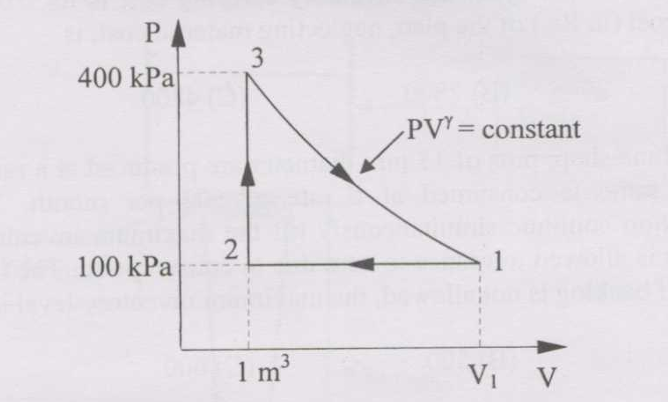
\includegraphics[width=0.8\textwidth]{Fig 10.png}
    \caption{}
    \label{fig:question74,75}
\end{figure}

\item The above cycle is represented on T–S plane by
\begin{multicols}{2}
\begin{enumerate}

\item
\begin{figure}[H]
    \centering
    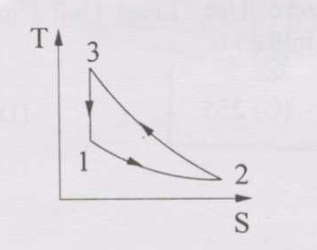
\includegraphics[width=0.3\textwidth]{Fig 11.png}
    \caption{}
    \label{fig:question74}
\end{figure}

\item 
\begin{figure}[H]
    \centering
    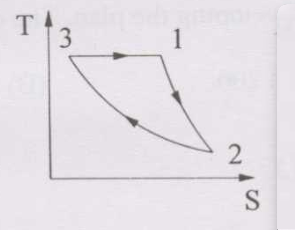
\includegraphics[width=0.3\textwidth]{Fig 12.png}
    \caption{}
    \label{fig:question74}
\end{figure}

\item 
\begin{figure}[H]
    \centering
    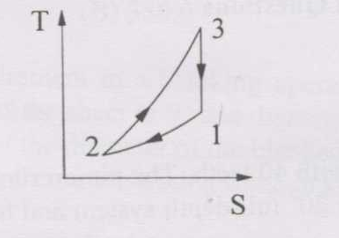
\includegraphics[width=0.3\textwidth]{Fig 13.png}
    \caption{}
    \label{fig:question74}
\end{figure}

\item 
\begin{figure}[H]
    \centering
    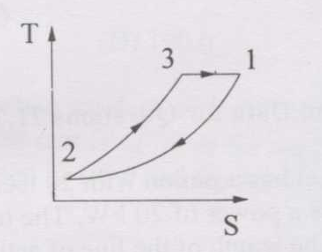
\includegraphics[width=0.3\textwidth]{Fig 14.png}
    \caption{}
    \label{fig:question74}
\end{figure}

\end{enumerate}
\end{multicols}
\hfill (GATE ME 2007)

\item If the specific heats of the working fluid are constant and the value of specific heat ratio $ \gamma = 1.4 $, the thermal efficiency (%) of the cycle is
\begin{multicols}{4}
\begin{enumerate}
\item 21
\item 40.9
\item 42.6
\item 59.7
\end{enumerate}
\end{multicols}
\hfill (GATE ME 2007)

\begin{center}
\textbf{Linked Answer Questions: Q.76 to Q.85 carry two marks each.}
\end{center}
\textbf{Statement for Linked Answer Questions 76 and 77:} 

Consider a steady incompressible flow through a channel as shown below.

\begin{figure}[H]
    \centering
    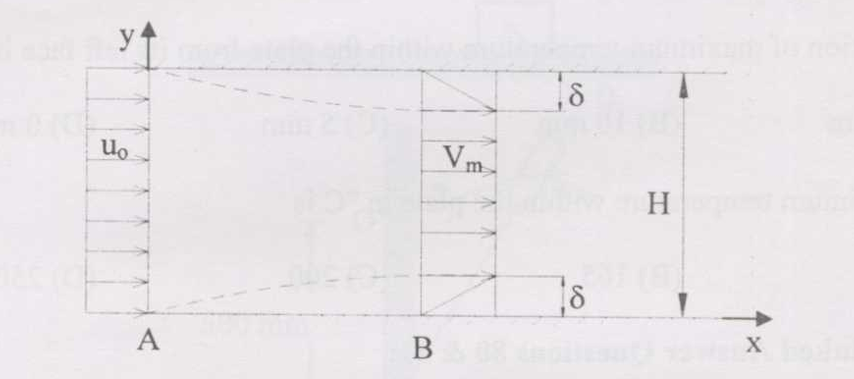
\includegraphics[width=0.8\textwidth]{Fig 15.png}
    \caption{}
    \label{fig:question76,77}
\end{figure}

The velocity profile is uniform with a value of $ U_0 $ at the inlet section A.  
The velocity profile at section B downstream is:

$u =
\begin{cases}
V_m \frac{y}{\delta}, & 0 \leq y \leq \delta \\
V_m, & \delta < y < H - \delta \\
V_m \frac{H - y}{\delta}, & H - \delta \leq y \leq H
\end{cases}
$

\item The ratio $ V_m / U_0 $ is
\begin{multicols}{2}
\begin{enumerate}
\item $ 1 - \frac{\delta}{H} $
\item 1
\item $ \frac{1}{1 + \frac{\delta}{H}} $
\item $ \frac{1}{[1 - \frac{\delta}{H}]^2} $
\end{enumerate}
\end{multicols}
\hfill (GATE ME 2007)

\item The ratio $\\frac{P_A - P_B}{\frac{1}{2} \rho u_0^2}$(where $ P_A $ and $ P_B $ are the pressures at section A and B respectively, and $ \rho $ is the density of the fluid) is
\begin{multicols}{2}
\begin{enumerate}
\item $ \frac{1}{(1 - (\delta / H))^2} - 1 $
\item $ \frac{1}{[1 - (\delta / H)]^2} $
\item $ \frac{1}{(1 - (2\delta / H))^2} - 1 $
\item $ \frac{1}{1 + (\delta / H)} $
\end{enumerate}
\end{multicols}
\hfill (GATE ME 2007)

\textbf{Statement for Linked Answer Questions 78 and 79:} 

Consider steady one-dimensional heat flow in a plate of 20 mm thickness with a uniform heat generation of 80 MW/m$^3$. The left and right faces are kept at constant temperatures of 160°C and 120°C respectively. The plate has a constant thermal conductivity of 200 W/m·K.

\item The location of maximum temperature within the plate from its left face is
\begin{multicols}{4}
\begin{enumerate}
\item 15 mm
\item 10 mm
\item 5 mm
\item 0 mm
\end{enumerate}
\end{multicols}
\hfill (GATE ME 2007)

\item The maximum temperature within the plate in °C is
\begin{multicols}{4}
\begin{enumerate}
\item 160
\item 165
\item 200
\item 250
\end{enumerate}
\end{multicols}
\hfill (GATE ME 2007)

\textbf{Statement for Linked Answer Questions 80 and 81:}

A machine frame is subjected to a horizontal force of 600 N parallel to the z-direction.

\begin{figure}[H]
    \centering
    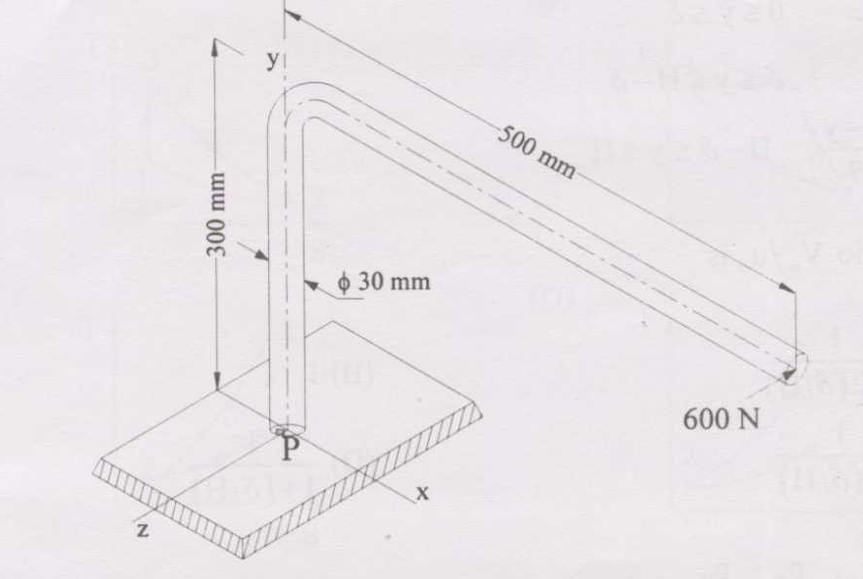
\includegraphics[width=0.8\textwidth]{Fig 16.png}
    \caption{}
    \label{fig:question80,81}
\end{figure}

\item The normal and shear stresses in MPa at point P are respectively
\begin{multicols}{2}
\begin{enumerate}
\item 67.9 and 56.6
\item 56.6 and 67.9
\item 67.9 and 0.0
\item 0.0 and 56.6
\end{enumerate}
\end{multicols}
\hfill (GATE ME 2007)

\item The maximum principal stress in MPa and the orientation of the corresponding principal plane in degrees are respectively
\begin{multicols}{2}
\begin{enumerate}
\item -32.0 and -29.52
\item 100.0 and 60.48
\item -32.0 and 60.48
\item 100.0 and -29.52
\end{enumerate}
\end{multicols}
\hfill (GATE ME 2007)

\textbf{Statement for Linked Answer Questions 82 and 83:} 

A quick return mechanism is shown. The crank OS is driven at 2 rev/s in counter-clockwise direction.

\begin{figure}[H]
    \centering
    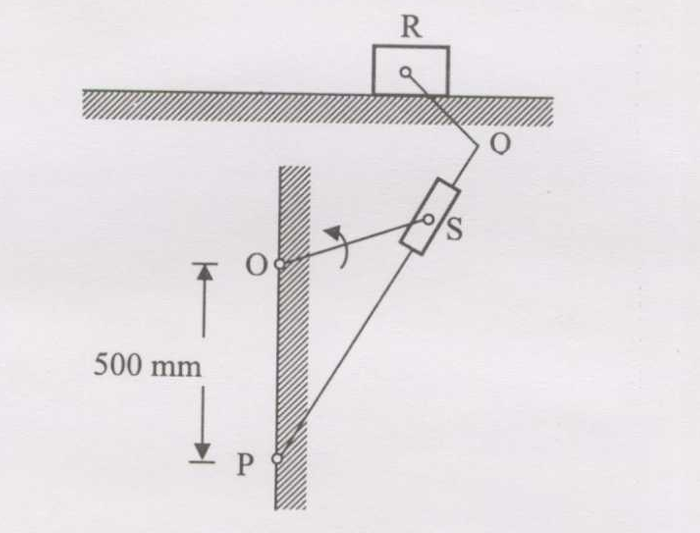
\includegraphics[width=0.8\textwidth]{Fig 17.png}
    \caption{}
    \label{fig:question82,83}
\end{figure}

\item If the quick return ratio is 1:2, then the length of the crank in mm is
\begin{multicols}{4}
\begin{enumerate}
\item 250
\item $ 250\sqrt{3} $
\item 500
\item $ 500\sqrt{3} $
\end{enumerate}
\end{multicols}
\hfill (GATE ME 2007)

\item The angular speed of PQ in rev/s when the block R attains maximum speed during forward stroke is
\begin{multicols}{4}
\begin{enumerate}
\item $ \frac{1}{3} $
\item $ \frac{2}{3} $
\item 2
\item 3
\end{enumerate}
\end{multicols}
\hfill (GATE ME 2007)

\textbf{Statement for Linked Answer Questions 84 and 85:}

A low carbon steel bar of 147 mm diameter with a length of 630 mm is being turned with uncoated carbide insert. The observed tool lives are 24 min and 12 min for cutting velocities of 90 m/min and 120 m/min respectively. The feed and depth of cut are 0.2 mm/rev and 2 mm respectively. Use the unmachined diameter to calculate the cutting velocity.

\item When tool life is 20 min, the cutting velocity in m/min is
\begin{multicols}{4}
\begin{enumerate}
\item 87
\item 97
\item 107
\item 114
\end{enumerate}
\end{multicols}
\hfill (GATE ME 2007)

\item Neglect over-travel or approach of the tool. When tool life is 20 min, the machining time in min for a single pass is
\begin{multicols}{4}
\begin{enumerate}
\item 5
\item 10
\item 15
\item 20
\end{enumerate}
\end{multicols}
\hfill (GATE ME 2007)

\end{enumerate}
\end{document}